\subsubsection{主页}

标题栏显示项目标题和登录状态,左侧是标签页切换按钮,右侧是主页大标题和登录、退出软件两个按钮,见图\ref{fig:home}。

\begin{figure}[H]
    \centering
    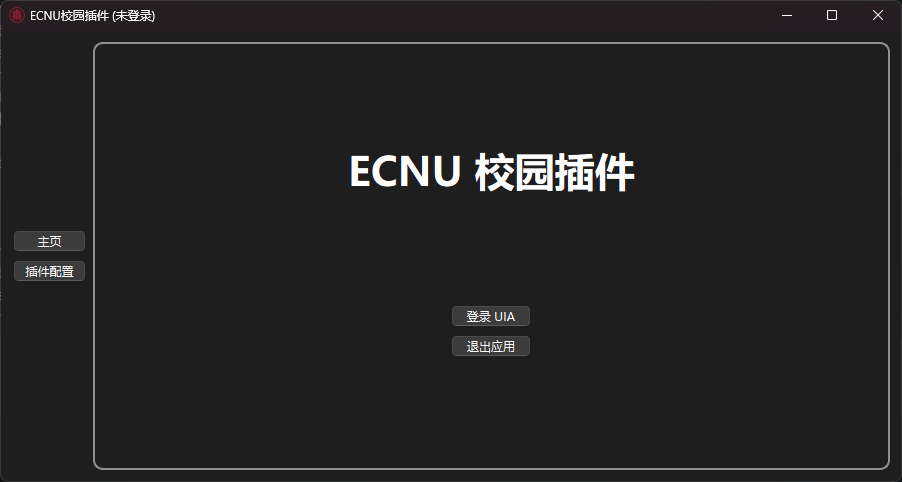
\includegraphics[width=0.8\textwidth]{img/home}
    \caption{主页}
    \label{fig:home}
\end{figure}

\subsubsection{插件配置页面}\label{subsubsec:gui-plugin-config}

插件配置页面右侧框中左侧的列表是插件选择,鼠标单击即可进入各个插件的配置界面,如图\ref{fig:plugin-config-gui} 中红框所示。

在每个插件的配置界面,会根据插件注册时提供的配置项生成可交互配置界面。

\begin{figure}[H]
    \centering
    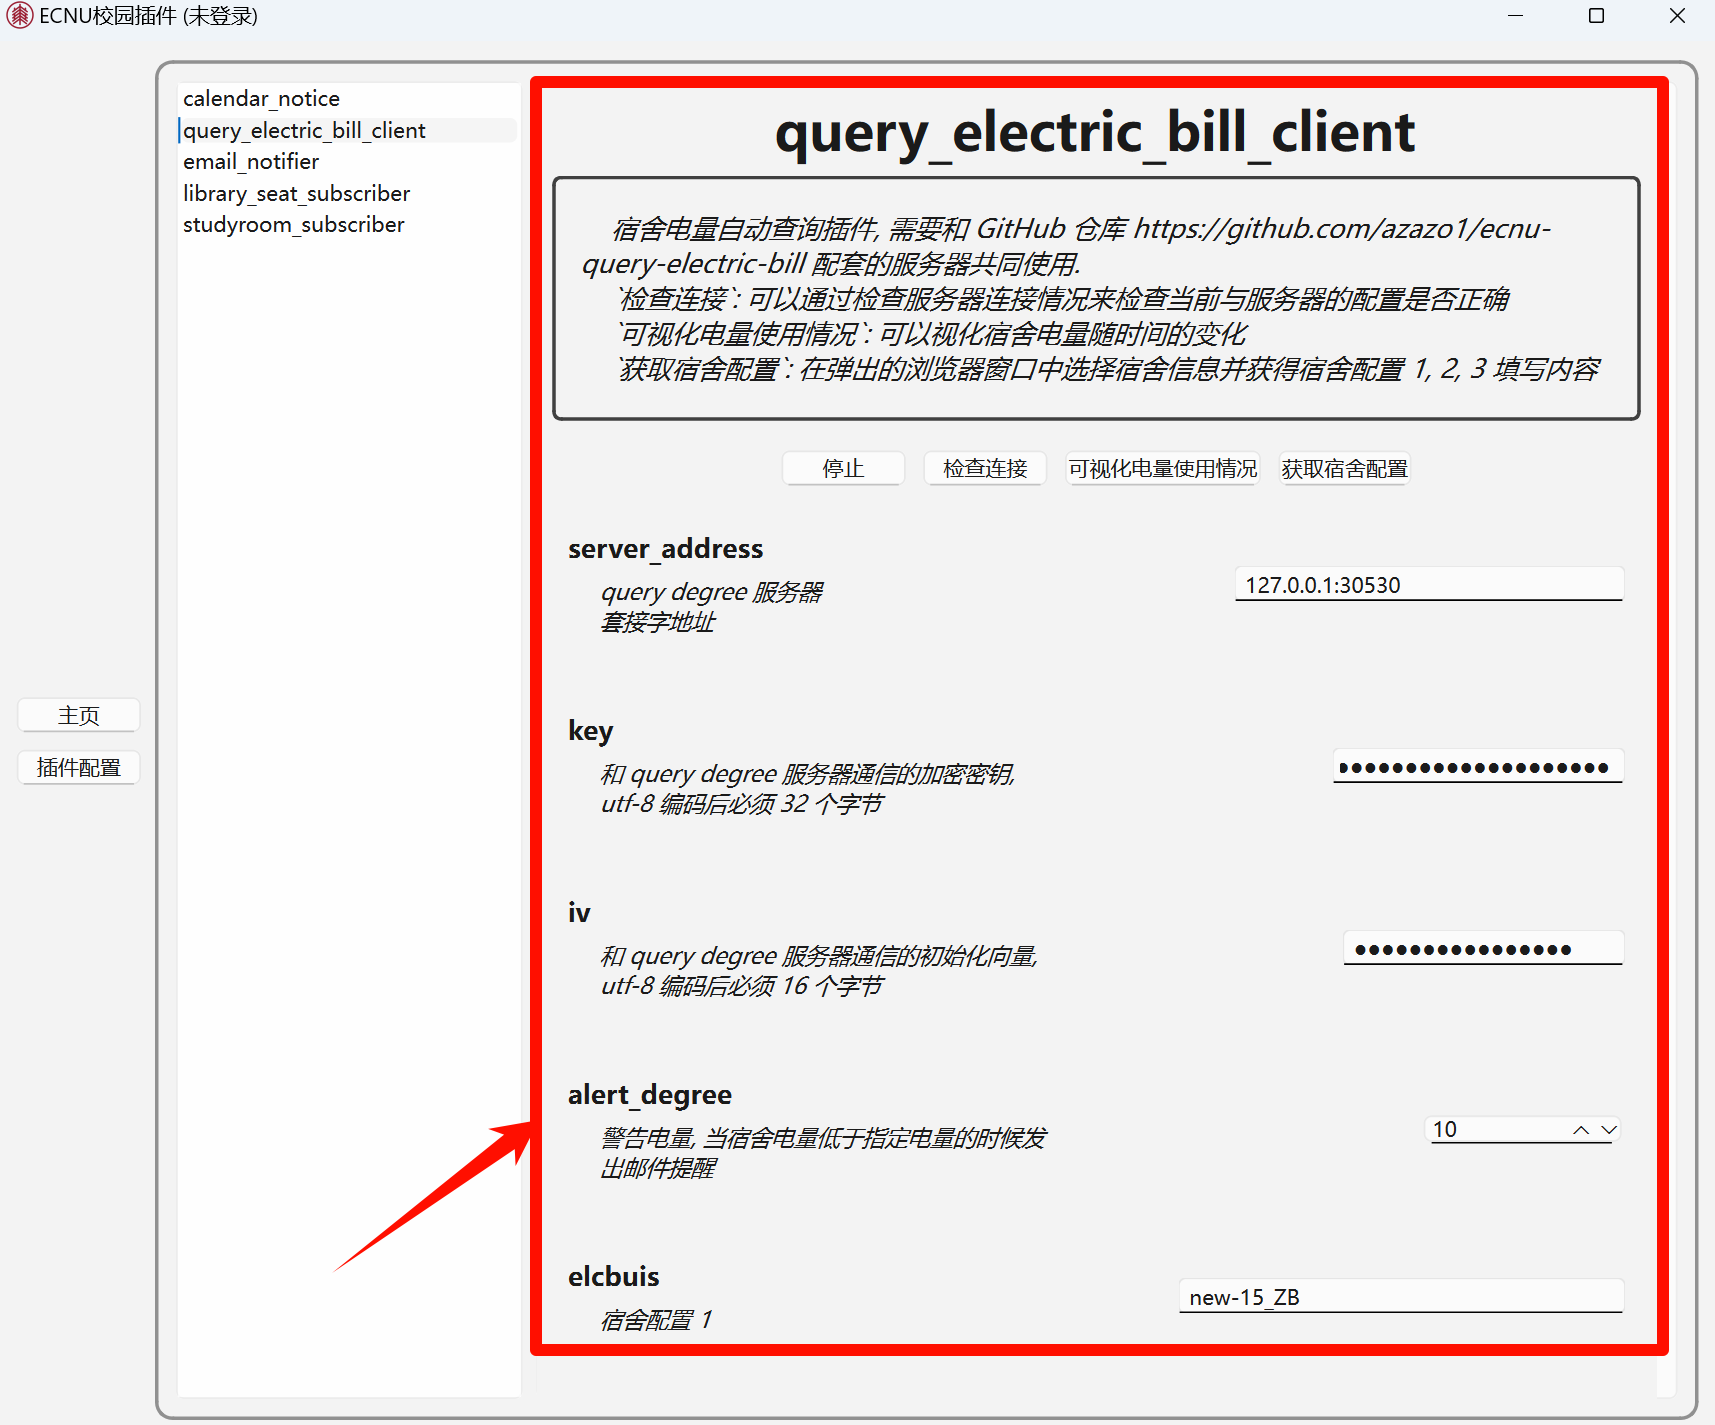
\includegraphics[width=0.8\textwidth]{img/plugin_config_gui}
    \caption{插件配置界面示例}
    \label{fig:plugin-config-gui}
\end{figure}

\subsubsection{系统托盘图标}

启动项目后,托盘中会出现 ECNU 图标,鼠标悬停可以查看当前的登录状态,使用鼠标右键显示菜单。
见图\ref{fig:tray-icon}、图\ref{fig:tray-icon-hover}、图\ref{fig:tray-icon-menu}。

\begin{figure}[H]
    \centering
    \begin{subfigure}[b]{0.3\textwidth}
        \centering
        
\includegraphics{img/tray_icon}
        \caption{系统托盘图标}
        \label{fig:tray-icon}
    \end{subfigure}
    \hspace{0.06\textwidth}
    \begin{subfigure}[b]{0.3\textwidth}
        \centering
        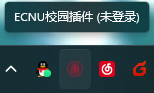
\includegraphics{img/tray_icon_hover}
        \caption{鼠标悬浮显示状态}
        \label{fig:tray-icon-hover}
    \end{subfigure}
    \begin{subfigure}[b]{0.3\textwidth}
        \centering
        
\includegraphics{img/tray_icon_menu}
        \caption{右键显示菜单}
        \label{fig:tray-icon-menu}
    \end{subfigure}
\end{figure}

